{Given the graph of $\fp$, identify the intervals of increasing and decreasing as well as the $x$ coordinates of the relative extrema.\\
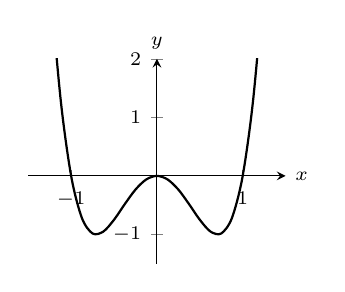
\begin{tikzpicture}
\begin{axis}[width=.4\textwidth,tick label style={font=\scriptsize },
	axis y line=middle,axis x line=middle,
    ymin=-1.5,ymax=2,
	xmin=-1.5,xmax=1.5,name=myplot]
\addplot [{\colorone},smooth,thick,domain=-1.5:1.5] {4*x^2*(x^2-1)};
\end{axis}
\node [right] at (myplot.right of origin) {\scriptsize $x$};
\node [above] at (myplot.above origin) {\scriptsize $y$};
\end{tikzpicture}}
{decreasing on $(-1,1)$,\\
increasing on $(-\infty,-1)\cup(1,\infty)$;\\
local maxima when $x=-1$,\\
local minima when $x=1$.}
